% !TEX root = ../thesis.tex
%
\chapter{Ablation Study}
In this chapter, we investigate the individual contributions of key factors influencing the performance and behavior of our proposed method.
Specifically, we focus on the effects of bias strength, the number of sensitive attributes, and the number of decisions on the system's overall functionality.
These factors are central to understanding the robustness and scalability of our approach.

\section{Bias Strength}
First, we will evaluate the sensitivity of the method to varying levels of inherent bias in the training data.
For this experiment, we selected the simulated \textit{cancer screening} model due to its easily adjustable parameters.
While the model remains largely consistent with the version depicted in figure \ref{fig:cancer_screening},
we modify the bias strength at the gateway following the activity \textit{assess screening eligibility},
which determines transitions to \textit{collect patient history} and \textit{refuse screening}.
Before, the probabilities to transition to either of these activities were split 70/30, depending on the gender of the patient.
In this analysis, we vary the probabilities incrementally from $0.5$ (perfectly equal) to $1.0$ (entirely biased) in steps of $0.05$.
For each step, we perform 5-fold cross-validation and  accuracy and 
The corresponding results are presented in the figures \ref{fig:ablation_bias_accuracy} and \ref{fig:ablation_bias_fairness}.

\begin{figure}[h!]
    \centering
    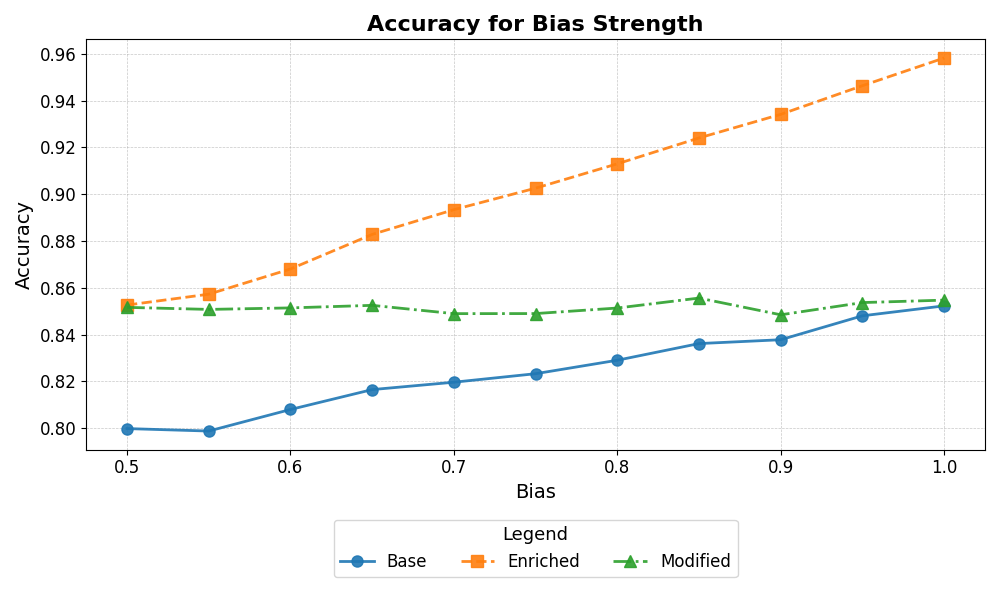
\includegraphics[width=0.9\textwidth]{gfx/ablation_bias_accuracy.png}
    \caption{Impact of varying bias strength on the accuracy.}
    \label{fig:ablation_bias_accuracy}
\end{figure}

\begin{figure}[h!]
    \centering
    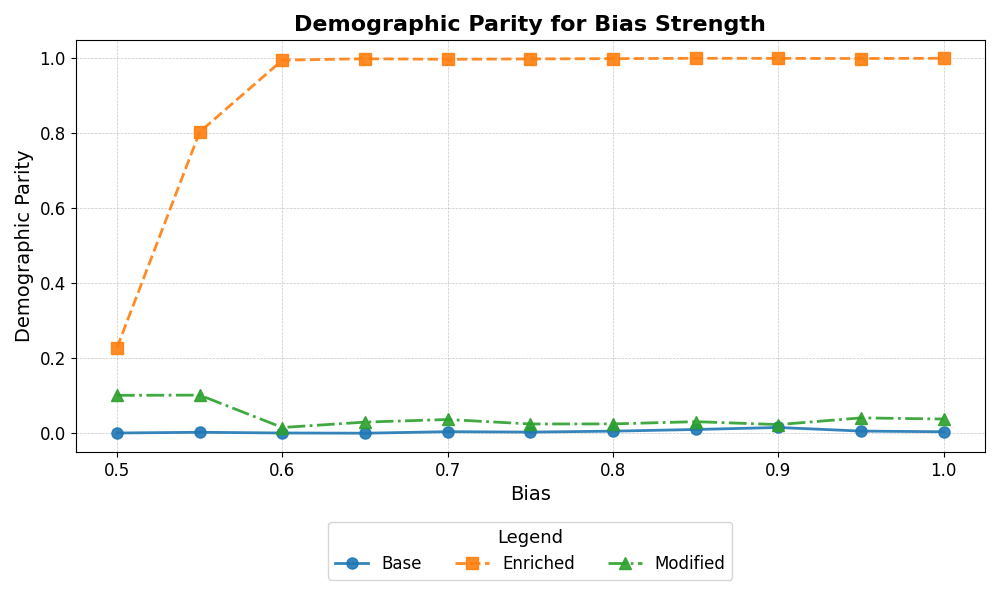
\includegraphics[width=0.9\textwidth]{gfx/ablation_bias_fairness.png}
    \caption{Impact of varying bias strength on the demographic parity.}
    \label{fig:ablation_bias_fairness}
\end{figure}




\section{Number of sensitive Attributes}
% attributes explanation

% describe the modified cs model

% for a single split, plot 1, 5, 10, 25, 50, 100

\begin{figure}[h!]
    \centering
    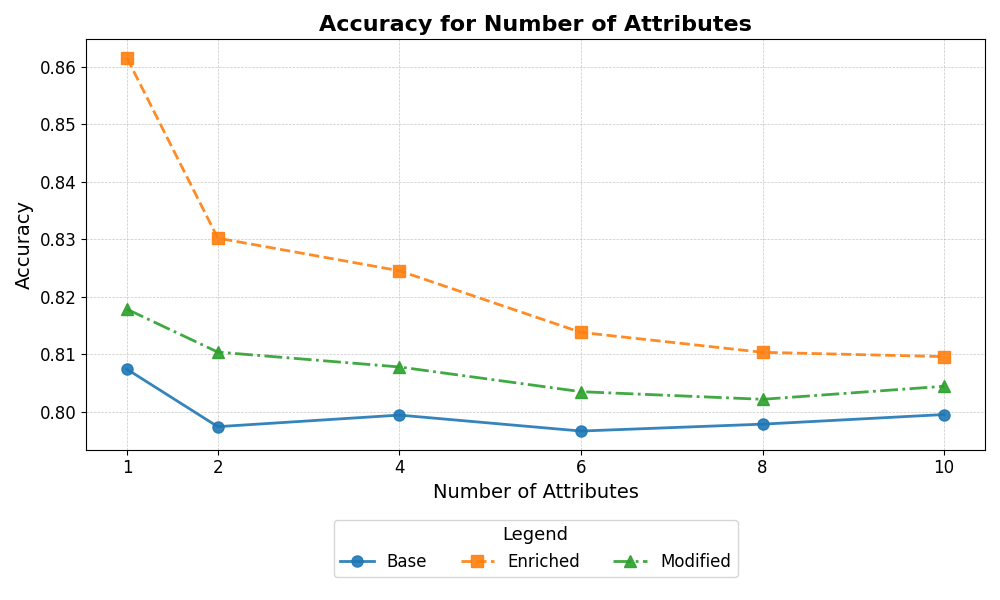
\includegraphics[width=0.9\textwidth]{gfx/ablation_attributes_accuracy.png}
    \caption{Impact of varying number of sensitive attributes on the accuracy}
    \label{fig:ablation_attributes_accuracy}
\end{figure}

\begin{figure}[h!]
    \centering
    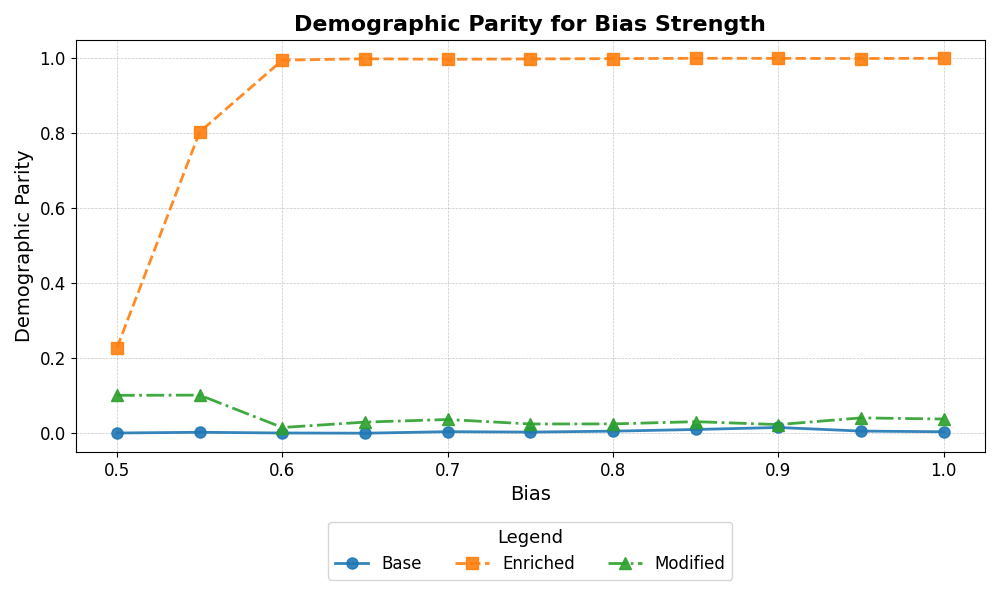
\includegraphics[width=0.9\textwidth]{gfx/ablation_bias_fairness.png}
    \caption{Impact of varying number of sensitive attributes on the demographic parity.}
    \label{fig:ablation_attributes_fairness}
\end{figure}

\section{Number of Biased Decisions}

\begin{figure}[h!]
    \centering
    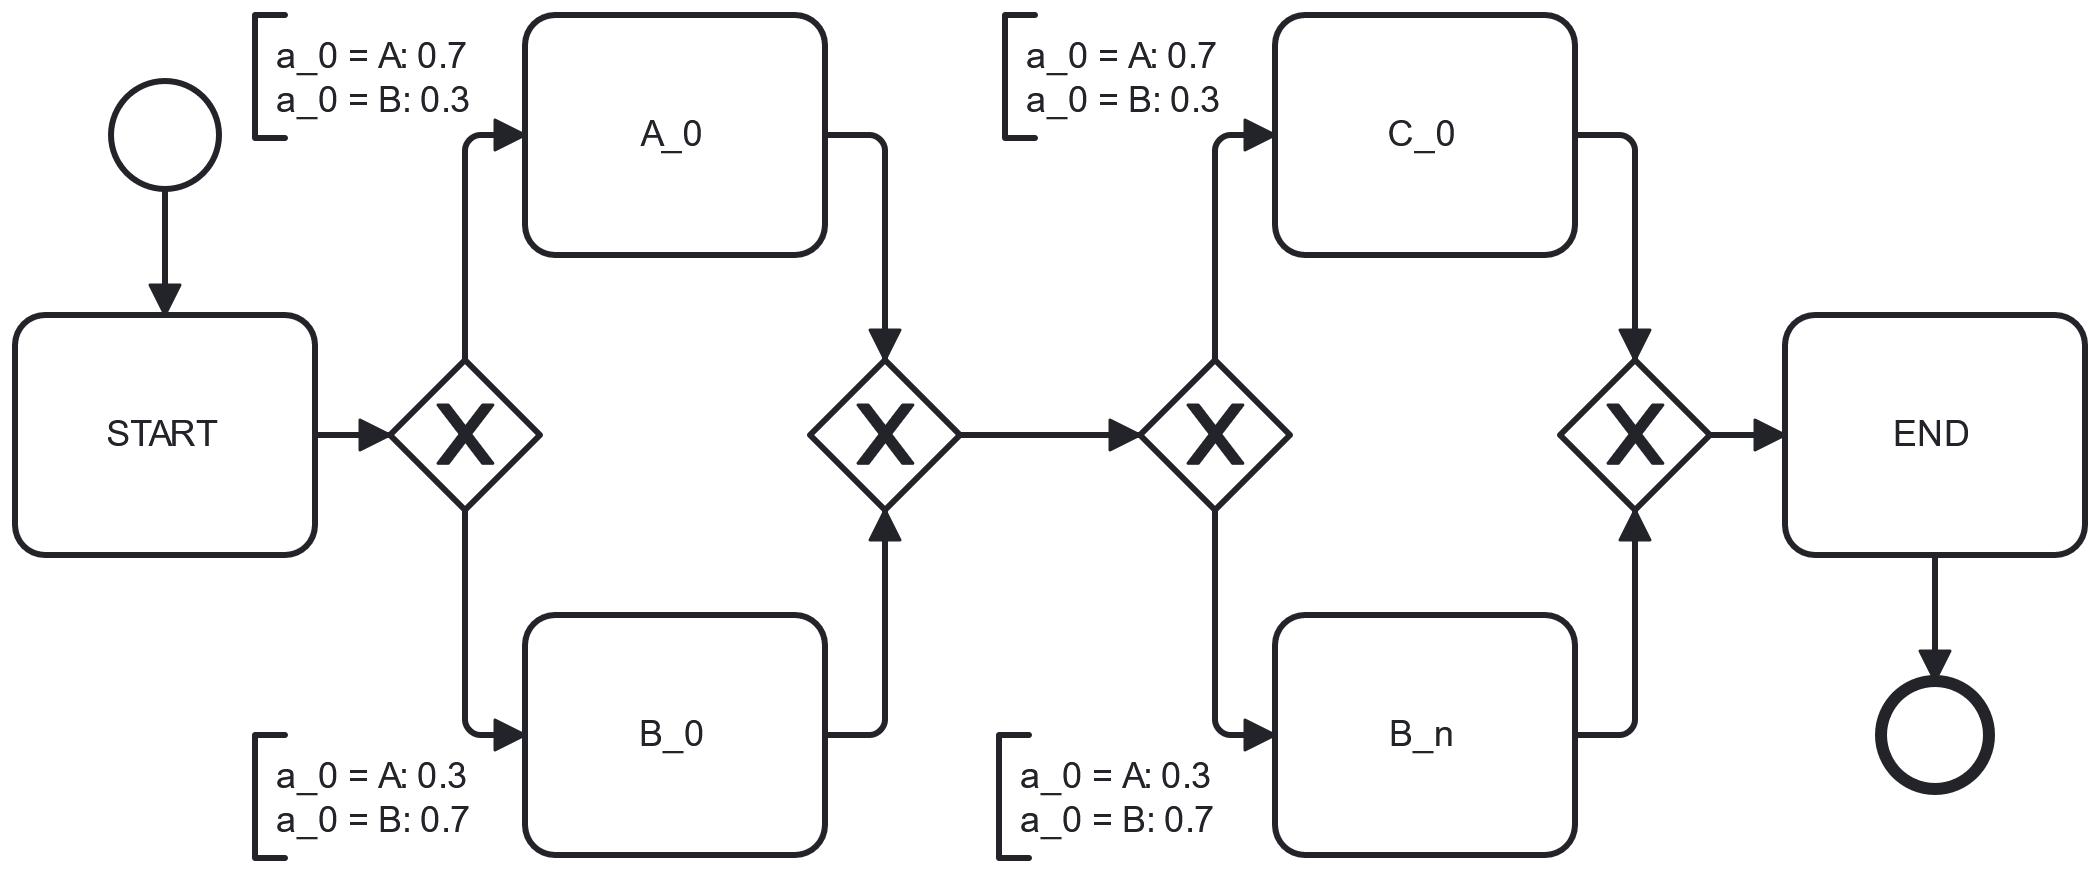
\includegraphics[width=\textwidth]{gfx/ablation_decision.png}
    \caption{The shortened process model, used for the ablation study of number of biased decisions.
    The ... in the sequence flow indicates where the rest of the events
    $A\_i, B\_i$ are, with $i \in \{1,\}$.
    These follow the same structure as shown for $A\_0, B\_0$ and $A\_n, B\_$}
    \label{fig:ablation_decision_model}
\end{figure}

\begin{figure}[h!]
    \centering
    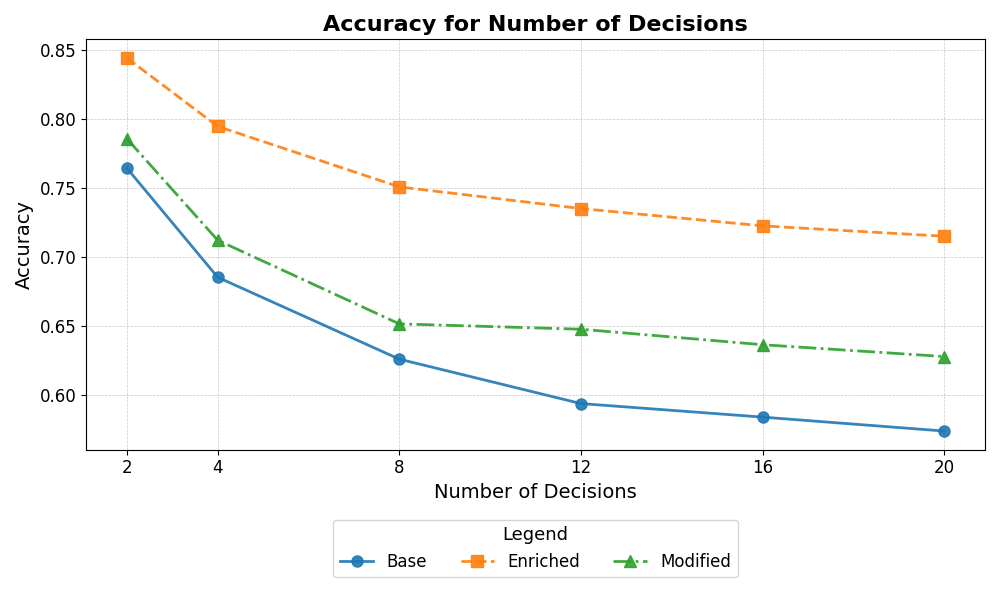
\includegraphics[width=0.9\textwidth]{gfx/ablation_decisions_accuracy.png}
    \caption{Impact of varying number of biased decisions on the accuracy.}
    \label{fig:ablation_bias_accuracy}
\end{figure}

\begin{figure}[h!]
    \centering
    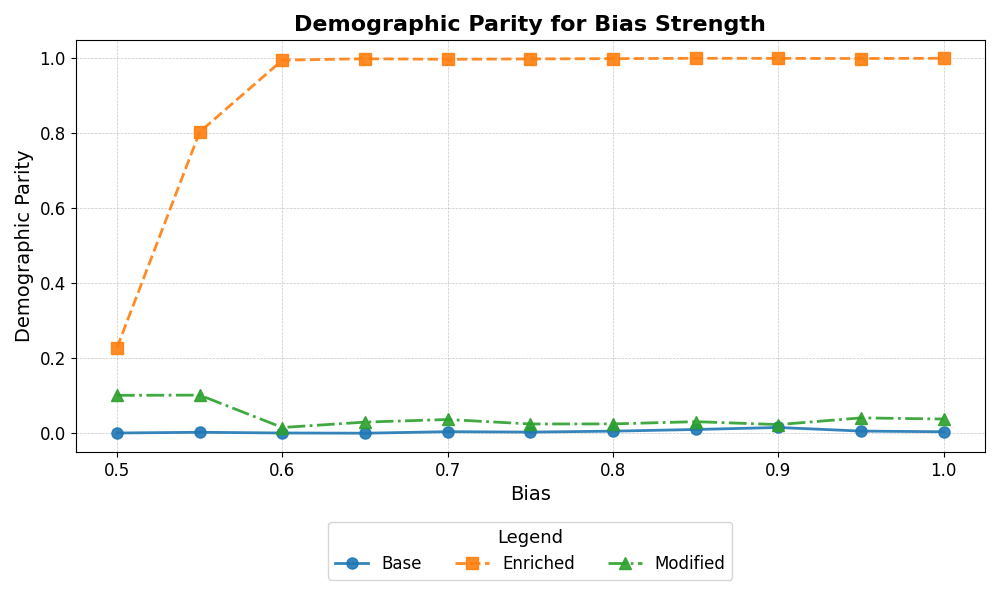
\includegraphics[width=0.9\textwidth]{gfx/ablation_decisions_fairness.png}
    \caption{Impact of varying number of biased decisions on the demographic parity.}
    \label{fig:ablation_bias_fairness}
\end{figure}

% describe the model: 2 rows of events

% evaluate x numbers of decision points